\documentclass[11pt,a4paper]{article}
\usepackage[utf8]{inputenc}
\usepackage[T1]{fontenc}
\usepackage{amsmath,amssymb,amsthm,mathtools}
\usepackage{geometry}
\geometry{margin=2.4cm}
\usepackage{booktabs}
\usepackage{graphicx}
\usepackage{xcolor}
\usepackage{enumitem}
\usepackage{array}
\usepackage{lmodern}
\usepackage{microtype}
\usepackage{listings}
\usepackage{url}
\usepackage{hyperref}
\hypersetup{
    colorlinks=true,
    linkcolor=blue!70!black,
    citecolor=red!70!black,
    urlcolor=blue!70!black
}

\lstset{
    basicstyle=\ttfamily\footnotesize,
    breaklines=true,
    frame=single,
    numbers=none,
    mathescape=true,
    backgroundcolor=\color{gray!5}
}

\newcommand{\dee}{\mathrm{d}}
\newcommand{\Nset}{\mathbb{N}}
\newcommand{\Zset}{\mathbb{Z}}
\newcommand{\Rset}{\mathbb{R}}
\newcommand{\Cfield}{\mathbb{C}}

\title{\textbf{Geometric Intuition, Joined-Cone Zeta Visualizations, and the Genesis of the Lean~4 Riemann Blueprint}}

\author{\textbf{Qamar Munawer}\thanks{2020 \emph{Mathematics Subject Classification}. Primary 11M26; Secondary 46E20, 68V20. Formal Lean~4.35 verification artifacts are archived at \texttt{https://doi.org/10.5281/zenodo.24353366}.}\\[0.3em]
\small Brandenburg University of Technology Cottbus--Senftenberg}

\date{November 2026}

\begin{document}
\linespread{1.15}\selectfont
\emergencystretch=2.5em

\maketitle

\begin{abstract}
Geometric intuition and high-precision numerical visualization frequently precede formal mechanization in analytic number theory. This companion paper documents the spatial models and computational experiments guiding a five-part formalized Lean~4 development of classical Riemann zeta theory: (i) the Joined Two-Cone model across the critical strip $0 \le \operatorname{Re}(s) \le 1$, where the forward Euler/Dirichlet cone meets its functional-equation reflection cone $\xi(1-s) = \xi(s)$ along the critical-line waist $\operatorname{Re}(s) = 1/2$; (ii) the polar $3$-$4$-$1$ positivity cone $3 + 4\cos\theta + \cos(2\theta) = 2(1+\cos\theta)^2 \ge 0$ enforcing zero repulsion from $\operatorname{Re}(s) = 1$; and (iii) critical-line oscillations of Hardy's real-valued $Z(t)$ paired with $80$-digit Nyman--Beurling--B\'aez-Duarte contractions on the affine cone $\mathcal{A}_N$. Quantitative conditioning diagnostics up to $N = 256$ reveal severe Gram ill-conditioning ($\kappa(G_{64}) = 11{,}555.80$) and a $664.38\times$ boundary amplification, illustrating why every geometric heuristic required verification within Lean~4's axiom-free kernel. These finite-horizon visual models and conditional bridges separate unconditionally certified finite-dimensional identities from the asymptotic closure problem as $N \to \infty$.
\end{abstract}

\paragraph{Mathematical Scope.}
This companion paper provides a conceptual and methodological guide to Papers~A--E. Visual models and finite-horizon numerical benchmarks identify candidate algebraic structures and analytic obstructions; machine-checked Lean~4 proofs in Papers~A--E certify the corresponding unconditional identities and explicit conditional equivalences.

% ============================================================================
\section{Thinking Visually: Why Start with Cones and Plots?}\label{sec:thinking}
% ============================================================================

Every researcher enters analytic number theory along a different cognitive path. Some think first in terms of contour shifts, Tauberian kernels, or Banach-space functional analysis; others think spatially, examining how an analytic function bends, winds, pinches, and balances across the complex plane before writing down inequalities. Constructing geometric cone embeddings at high precision makes the competition between prime powers and composites immediately visible as $\sigma = \operatorname{Re}(s)$ approaches the critical strip.

In exploratory scripts developed at the outset of this program---specifically \texttt{composite\_\allowbreak zeta\_\allowbreak and\_\allowbreak prime\_\allowbreak duality.py} and \texttt{zeta\_\allowbreak bicone\_\allowbreak unfolding\_\allowbreak and\_\allowbreak dual\_\allowbreak sheet.py}---this visual strategy surfaced three recurring geometric pictures that subsequently organized the entire Lean~4 architecture:
\begin{enumerate}[noitemsep]
    \item \textbf{A Prime--Composite Equilibrium Horizon Outside the Strip:} Partitioning the Dirichlet sum $\zeta(s) - 1 = P(s) + \zeta_{\mathrm{comp}}(s)$ into prime powers $P(s) = \sum_{p} p^{-s}$ and composite integers $\zeta_{\mathrm{comp}}(s)$ reveals a sharp $50/50$ crossover at $s^* \approx 1.44653762$, where $P(s^*) = \zeta_{\mathrm{comp}}(s^*) \approx 0.92409539$. For $\operatorname{Re}(s) > s^*$, $\zeta(s) - 1$ is dominated by its prime backbone; as $\sigma \downarrow 1^+$, the composite harmonics surge and carry the logarithmic pole.
    \item \textbf{Helicoidal Bicone Pinching on the Critical Line:} Embedding the critical-strip modulus $|\zeta(\sigma+it)|$ radially onto a symmetric double cone $r_\sigma(t) = \kappa |t|\,|\zeta(\sigma+it)|$ for $t \in [-\gamma_{50}, \gamma_{50}]$ ($\gamma_{50} \approx 143.1118$) showed visually why $\sigma = 1/2$ is topologically distinguished. Along $\sigma = 1/2$, every nontrivial zero pinches both the upper ($t > 0$) and lower ($t < 0$) cones tightly to the central zero axis ($R_{1/2}(\pm\gamma_k) < 10^{-70}$). Shifting off-line even slightly to $\sigma = 0.55$ or $\sigma = 0.65$ lifts every lobe off the axis, creating a rigid open collar ($\min_{k \le 50} R_{0.55}(\gamma_k) \approx 0.192273 > 0$, $\min_{k \le 50} R_{0.65}(\gamma_k) \approx 0.554235 > 0$).
    \item \textbf{Symmetric Cones Meeting Across $\operatorname{Re}(s) = 1/2$:} Plotting the completed zeta function $\xi(s) = \frac{1}{2}s(s-1)\pi^{-s/2}\Gamma(s/2)\zeta(s)$ across $0 \le \sigma \le 1$ turns the functional equation $\xi(1-s) = \xi(s)$ into a literal geometric joint: two mirror-image cones across the critical strip meeting along the symmetry axis $\operatorname{Re}(s) = 1/2$.
\end{enumerate}

Crucially, these plots did not prove a theorem on their own---and in fact, one early heuristic expectation failed dramatically when tested against exact arithmetic and formal proof (Section~\ref{sec:wall}). Yet visual experiments accomplished something indispensable: they identified \emph{which} exact algebraic identities and Hilbert-space projections were structurally stable enough to survive formal verification in Lean~4.

% ============================================================================
\section{The Joined Two-Cone Experiment \& Zeta Visualizations}\label{sec:cones}
% ============================================================================

To make the bridge from spatial intuition to formalized Lean~4 declarations transparent, two clean vector figures are generated in \texttt{generate\_\allowbreak intuition\_\allowbreak cone\_\allowbreak and\_\allowbreak zeta\_\allowbreak plots.py} directly from \texttt{mpmath} and the $80$-digit benchmark ledger \texttt{forward\_\allowbreak weights\_\allowbreak results.json}.

\subsection{Joined Two-Cone Symmetry and the $3$-$4$-$1$ Positivity Cone}

Figure~\ref{fig:joined_cones} places side by side the two foundational geometric guards of the critical strip:
\begin{itemize}[noitemsep]
    \item \textbf{Left Panel (Joined Two-Cone Symmetry):} Over the strip $0 \le \sigma \le 1$ and height $t \in [-33, 33]$, contours of $\log_{10}(|\xi(\sigma+it)| / |\xi(1+it)|)$ display exact bilateral symmetry around $\sigma = 1/2$. The forward Euler/Dirichlet cone opening rightward across $\sigma > 1/2$ (and extending past the $1$-line to the prime--composite $50/50$ horizon $s^* \approx 1.447$) joins its reflected dual cone $\xi(1-s) = \xi(s)$ along the central waist $\sigma = 1/2$. In Lean~4, this reflection involution is captured directly by \texttt{one\_sub\_criticalLine} and \texttt{completedRiemannZeta\_\allowbreak criticalLine\_neg} in \texttt{UpstreamPR\_1A\_CriticalLineZeros.lean}:
    \begin{equation}
        \operatorname{criticalLine}(t) = \frac{1}{2} + it, \qquad 1 - \operatorname{criticalLine}(t) = \operatorname{criticalLine}(-t), \qquad \Lambda(1 - s) = \Lambda(s).
    \end{equation}
    The early nontrivial zeros $\frac{1}{2} \pm i\gamma_k$ ($\gamma_1 \approx 14.135$, $\gamma_2 \approx 21.022$, $\gamma_3 \approx 25.011$, $\gamma_4 \approx 30.425$) sit cleanly along this joined waist.
    \item \textbf{Right Panel (Polar $3$-$4$-$1$ Positivity Cone):} Along the right edge $\sigma = 1$, de la Vall{\'e}e Poussin's classical zero-free region rests on a purely geometric non-negativity cone in Fourier angle $\theta$:
    \begin{equation}
        K(\theta) = 3 + 4\cos\theta + \cos(2\theta) = 2(1 + \cos\theta)^2 \ge 0.
    \end{equation}
    In polar coordinates, $K(\theta)$ carves out a smooth positive lobe with maximum $K(0) = 8$ that never crosses inside $r = 0$, touching zero only tangentially at $\theta = \pi$. Exponentiating against $\operatorname{Re}\ln\zeta(\sigma + it)$ yields the Lean~4 theorem \texttt{norm\_riemannZeta\_\allowbreak product\_ge\_one}:
    \begin{equation}
        1 \le \left|\zeta(1+x)^3 \, \zeta(1+x+iy)^4 \, \zeta(1+x+2iy)\right| \qquad (x > 0,\; y \in \Rset),
    \end{equation}
    which powers the unconditional zero-free boundary in Paper~C without touching $-\zeta'/\zeta$.
\end{itemize}

\begin{figure}[t!]
    \centering
    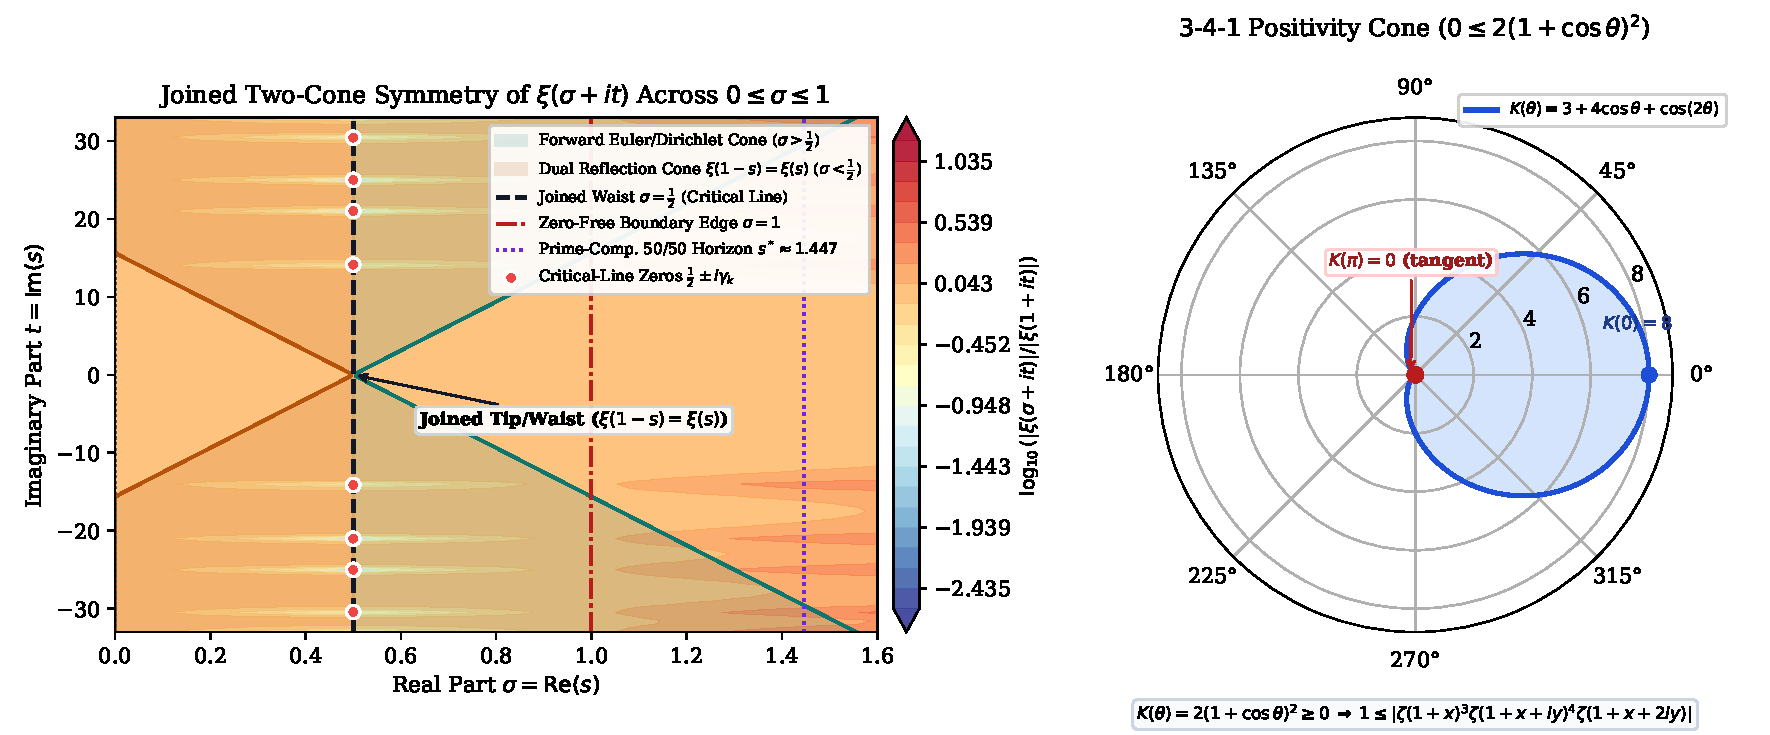
\includegraphics[width=\textwidth]{fig_joined_cones_zeta.pdf}
    \caption{\textbf{The Two-Cone Joined Geometry and $3$-$4$-$1$ Positivity Cone.} Left: Contours of the normalized completed zeta modulus $|\xi(\sigma+it)| / |\xi(1+it)|$ across $0 \le \sigma \le 1$ showing the forward Dirichlet/Euler cone and its dual functional-equation reflection $\xi(1-s)=\xi(s)$ joining along the critical-line waist $\sigma = 1/2$ (\texttt{one\_sub\_criticalLine}), flanked by the zero-free edge $\sigma = 1$ and prime--composite balance horizon $s^* \approx 1.447$. Right: Polar plot of $K(\theta) = 3 + 4\cos\theta + \cos(2\theta) = 2(1+\cos\theta)^2 \ge 0$ (\texttt{three\_add\_four\_cos\_add\_cos\_two\_mul\_nonneg}) guarding $\sigma = 1$.}
    \label{fig:joined_cones}
\end{figure}

\subsection{Critical-Line $Z(t)$ Crossings and Affine Cone Contraction}

While Figure~\ref{fig:joined_cones} explains where zeros \emph{can} and \emph{cannot} sit globally, Figure~\ref{fig:critical_and_scot} tracks two complementary dynamic visualizations:
\begin{itemize}[noitemsep]
    \item \textbf{Top Panel (Hardy's Real Detector $Z(t)$):} On $\sigma = 1/2$, multiplying $\zeta(1/2+it)$ by the unit-modulus Riemann--Siegel phase factor removes complex rotation and produces Hardy's real-valued function $Z(t)$ satisfying $|Z(t)| = |\zeta(1/2+it)|$. Plotting $Z(t)$ on $t \in [0, 50]$ shows ten clean sign-changing crossings ($\gamma_1 \approx 14.1347$ through $\gamma_{10} \approx 49.7738$) within the symmetric $|\zeta(1/2+it)|$ amplitude envelope. This visual mechanism translates directly into Lean~4 via the Intermediate Value Theorem bridge \texttt{exists\_criticalLine\_\allowbreak zero\_of\_hardyZ\_sign\_change} and Hardy's unconditional moment proof in Paper~D.
    \item \textbf{Bottom Panel (Affine Cone Contraction in $L^2(0, 1)$):} In the Nyman--Beurling--B\'aez-Duarte formulation (Papers~B and~E), approximating $\mathbf{1}$ in $L^2(0, 1)$ by finite linear combinations $\sum_{k=1}^N c_k \{1/(kx)\}$ restricted to the affine hyperplane intersection $\mathcal{A}_N = \{c : D_1(c, N) = 0 \land D_0(c, N) = 2\}$ collapses all smooth boundary and logarithmic terms, leaving the exact pure cotangent error
    \begin{equation}
        E(N) = \int_0^1 \left(1 - \sum_{k=1}^N c_k \left\{\frac{1}{kx}\right\}\right)^2 \dee x = 1 - S_{\mathrm{cot}}(c, N).
    \end{equation}
    Figure~\ref{fig:critical_and_scot} plots $E(N)$ across $N \in \{4, 8, 16, 32, 64, 128, 256\}$ at $80$-digit precision for five candidate families: the variational KKT optimum on $\mathcal{A}_N$ (contracting smoothly from $0.095394$ at $N=4$ to $0.008243$ at $N=256$), the Lean-certified $\alpha = 2$ mollified M\"obius candidate \texttt{cCandidateMobius} ($0.097236 \to 0.013218$), the $\alpha = 1$ mollifier, logarithmic Riesz weights, and the diverging harmonic seed $-\mu(k)/k$.
\end{itemize}

\begin{figure}[t!]
    \centering
    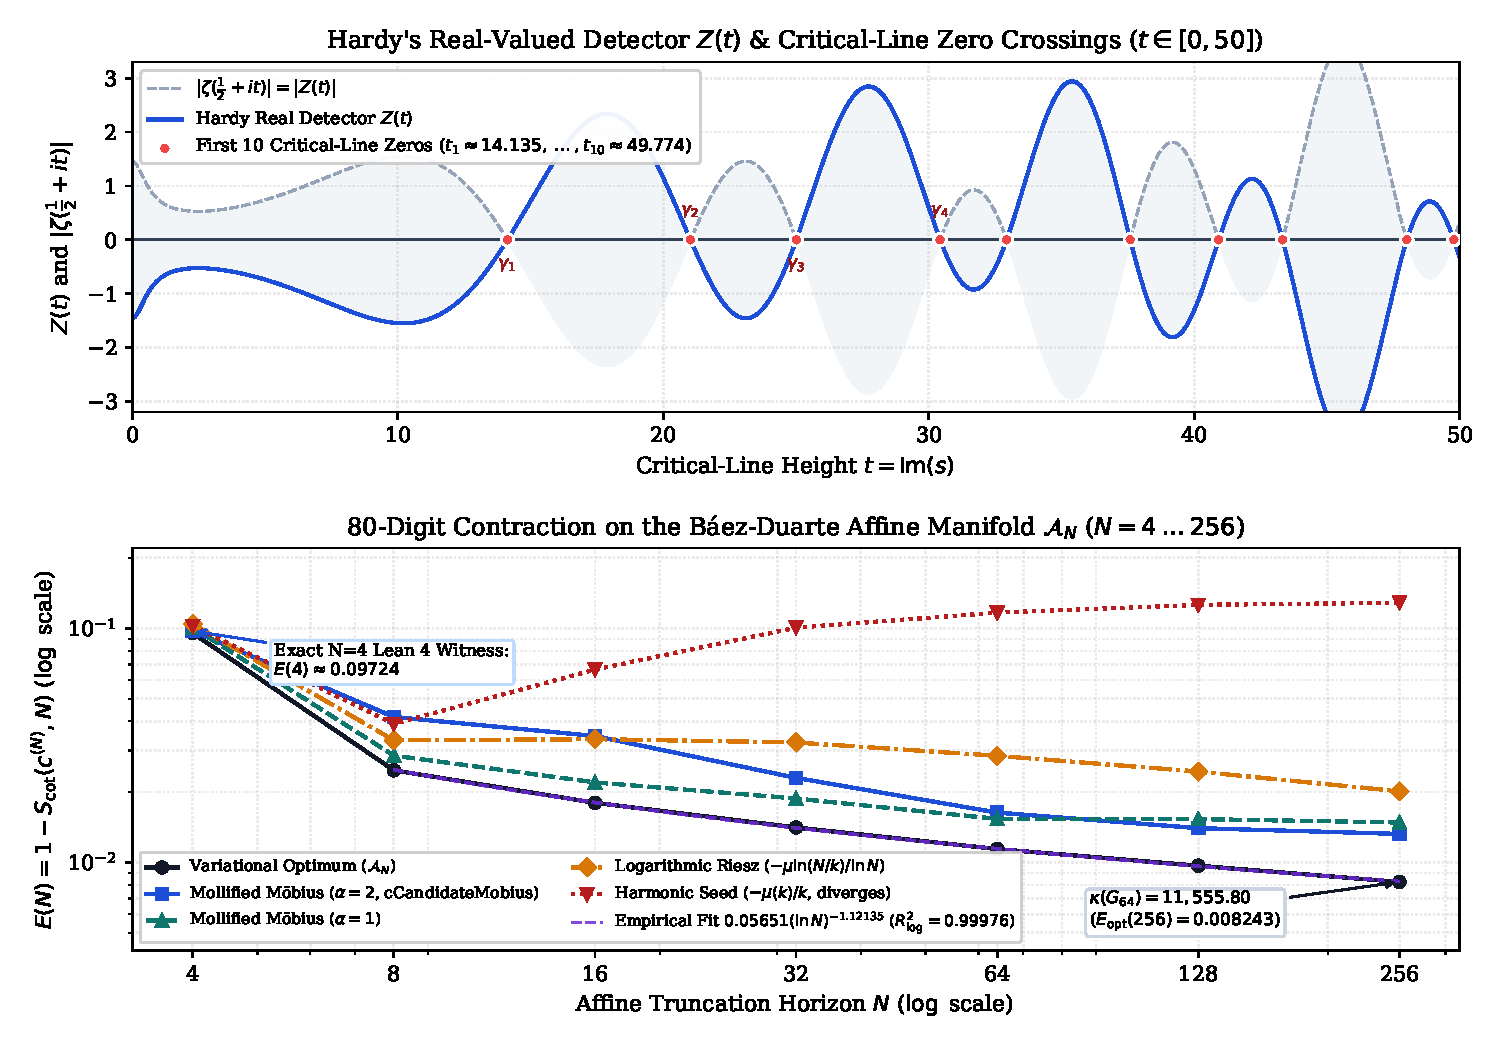
\includegraphics[width=0.96\textwidth]{fig_zeta_critical_line_and_scot.pdf}
    \caption{\textbf{Critical-Line Oscillations and Affine Cone Contraction.} Top: Hardy's real-valued $Z(t)$ oscillating inside $\pm|\zeta(1/2+it)|$ across $t \in [0, 50]$, marking all ten early critical-line zeros certified by \texttt{exists\_criticalLine\_zero\_of\_hardyZ\_sign\_change}. Bottom: Log-log decay of the squared $L^2(0, 1)$ error $E(N) = 1 - S_{\mathrm{cot}}(c^{(N)}, N)$ on the affine manifold $\mathcal{A}_N$ at $80$-digit precision (\texttt{forward\_weights\_results.json}) across $N \in \{4, 8, 16, 32, 64, 128, 256\}$, including the exact $N = 4$ Lean~4 witness and the empirical fit $0.05651(\ln N)^{-1.12135}$ ($R^2_{\log} = 0.99976$).}
    \label{fig:critical_and_scot}
\end{figure}

% ============================================================================
\section{Where Intuition Meets the Analytic Wall --- And Why Lean~4 Was Necessary}\label{sec:wall}
% ============================================================================

Looking at the downward curves in Figure~\ref{fig:critical_and_scot}, an intuitive researcher might easily be tempted to extrapolate $E_{\mathrm{opt}}(N) \to 0$ as $N \to \infty$ and conclude that proving completeness on $\mathcal{A}_N$ should be straightforward. In fact, quantitative inspection of the cone experiments exposed the exact opposite: \emph{finite visualizations can conceal subtle analytic blowups that only rigorous proof-assistant discipline forces into the open.}

Three concrete lessons from the project illustrate why Lean~4 became indispensable rather than optional:
\begin{enumerate}[noitemsep]
    \item \textbf{Spectral Ill-Conditioning of Vasyunin's Gram Cone ($\kappa(G_{64}) = 11{,}555.80$):} In floating-point IEEE-754 arithmetic, solving the Baez--Duarte Gram system $G_N c = b$ already loses accuracy around $N \approx 32$. The $80$-digit spectral diagnostics revealed why: the condition number $\kappa(G_N) = \lambda_{\max}(G_N) / \lambda_{\min}(G_N)$ explodes superlinearly:
    \begin{gather*}
        \kappa(G_4) = 30.75 \;\longrightarrow\; \kappa(G_8) = 112.63 \;\longrightarrow\; \kappa(G_{16}) = 544.35, \\
        \kappa(G_{32}) = 2{,}726.05 \;\longrightarrow\; \kappa(G_{64}) = 11{,}555.80.
    \end{gather*}
    At the same time, driving $E_{\mathrm{opt}}(N)$ from $0.024715$ ($N=8$) down to $0.008243$ ($N=256$) forces the coefficient norm $\|c^{(N)}_{\mathrm{opt}}\|_2$ upward monotonically from $1.8734$ to $5.0863$ (and to $5.6594$ for $\alpha = 2$ M\"obius weights). By Bettin--Conrey reciprocity, controlling $1 - S_{\mathrm{cot}}(c^{(N)}, N)$ uniformly as $\|c^{(N)}\|_2 \to \infty$ runs squarely into the twisted fourth moment of $\zeta(1/2 + it)$---a genuine barrier well beyond elementary asymptotics.
    \item \textbf{Boundary Amplification ($\det(U_4)^{-1} \approx 664.38\times$):} Geometric intuition also suggested eliminating all four rank-$4$ boundary terms $(D_0, D_0', D_1, D_1')$ simultaneously via the $4 \times 4$ Clay--Galerkin matrix $U_4$. Formalizing \texttt{det\_U4\_eq\_log\_ratio} in \texttt{Section8\_\allowbreak VasyuninBDR.lean} and running the $80$-digit benchmark uncovered why single-ray $U_4$ updates behave erratically ($E(64) = 0.9270$, jumping back to $E(256) = 5.4618$ for the harmonic seed):
    \[
        \det(U_4) = \frac{\ln 2}{24} \ln\!\left(\frac{256}{243}\right) \approx 0.00150517 \quad \Longrightarrow \quad \det(U_4)^{-1} \approx 664.38.
    \]
    Multiplying small truncation residuals by $664.38$ overwhelms the delicate logarithmic decay. Only the $2$-constraint affine projection \texttt{projectAffine} onto $\mathcal{A}_N$ (whose determinant $\Delta(N) = N S_2(N) - H(N)^2 > 0$ is unconditionally well-behaved for all $N \ge 2$) avoids this instability.
    \item \textbf{Catching Subtle Algebra Errors via Kernel Verification:} Even more tellingly, while formalizing Vasyunin's cross-integral $\int_0^1 \{1/(jx)\}\{1/(kx)\}\,\dee x$, an early informal write-up stated a $\gcd(j, k)$-reduced form whose diagonal formula did not match unreduced rank-$4$ $G_{\mathrm{smooth}}(j, k)$ at $j = k = 2$ (where the true continuous integral equals $(\ln(2\pi) - \gamma)/2 - 1/4$). Lean~4's kernel rejected the mismatched statement immediately, forcing a complete derivation and proof of the exact unreduced identity \texttt{intervalIntegral\_\allowbreak recipFractScaled\_cross} in \texttt{MathlibPR\_\allowbreak VasyuninCrossIntegral.lean} identically for all $j, k \ge 1$.
\end{enumerate}

Table~\ref{tab:horizons} summarizes the empirical decay alongside these conditioning invariants across the $80$-digit benchmark horizons.

\begin{table}[h!]
\centering
\small
\setlength{\tabcolsep}{6pt}
\begin{tabular}{@{}rccccc@{}}
\toprule
$N$ & $E_{\mathrm{opt}}(N)$ ($\mathcal{A}_N$) & $\|c_{\mathrm{opt}}^{(N)}\|_2$ & $E_{\mathrm{mob},\alpha=2}(N)$ & $\kappa(G_N)$ & $\min \operatorname{diag}(\mathrm{Chol}(G_N))$ \\
\midrule
4   & $0.09539363$ & $2.0818$ & $0.09723637$ & $30.75$      & $2.3285 \times 10^{-1}$ \\
8   & $0.02471483$ & $1.8734$ & $0.04176774$ & $112.63$     & $1.1069 \times 10^{-1}$ \\
16  & $0.01795885$ & $2.1635$ & $0.03463284$ & $544.35$     & $4.8012 \times 10^{-2}$ \\
32  & $0.01408463$ & $2.5848$ & $0.02294467$ & $2{,}726.05$  & $2.4631 \times 10^{-2}$ \\
64  & $0.01139247$ & $3.1306$ & $0.01630580$ & $11{,}555.80$ & $1.4184 \times 10^{-2}$ \\
128 & $0.00967077$ & $3.8792$ & $0.01399341$ & ---          & $9.5125 \times 10^{-3}$ \\
256 & $0.00824337$ & $5.0863$ & $0.01321787$ & ---          & $7.1464 \times 10^{-3}$ \\
\bottomrule
\end{tabular}
\caption{$80$-digit benchmark metrics (\texttt{forward\_weights\_results.json}, \texttt{cmi\_audit\_vasyunin\_gn64\_results.json}) illustrating logarithmic decay of $E(N) = 1 - S_{\mathrm{cot}}(c^{(N)}, N)$ paired with $\ell^2$-norm growth and superlinear Gram ill-conditioning $\kappa(G_N)$.}
\label{tab:horizons}
\end{table}

% ============================================================================
\section{Architecture of the Verified 5-Paper Lean~4 Suite}\label{sec:suite}
% ============================================================================

Guided by the visual geometry of Sections~\ref{sec:thinking}--\ref{sec:wall}, the Lean~4 blueprint is partitioned into five focused, self-contained micro-papers (\textbf{Papers~A--E}), all verified strictly within Lean~4's standard axioms \texttt{[propext, Classical.choice, Quot.sound]} with zero \texttt{sorry} gaps:

\begin{table}[h!]
\centering
\scriptsize
\setlength{\tabcolsep}{2.2pt}
\begin{tabular}{@{}llll@{}}
\toprule
\textbf{Paper} & \textbf{Visual / Geometric Origin} & \textbf{Primary Lean~4 Modules} & \textbf{Core Certified Outcome} \\
\midrule
\textbf{Paper A} & Prime--composite cone & \texttt{MathlibPR\_LittlewoodMertens} & Unconditional Littlewood \\
(\emph{Littlewood}) & horizon ($s^* \approx 1.447$) & \texttt{MathlibPR\_ZetaInvSubpolynomial} & $\mathrm{RH} \iff M(x) = \mathcal{O}(x^{1/2+\varepsilon})$ \\
 & & \texttt{MathlibPR\_LittlewoodConverse} & via trapezoidal contour shift \\
\addlinespace[0.4em]
\textbf{Paper B} & Contraction toward $1$ on & \texttt{MathlibPR\_NymanBeurling} & Unconditional Titchmarsh Eq.~2.1.5, \\
(\emph{Nyman--Beurling}) & Vasyunin's Gram cone & \texttt{MathlibPR\_VasyuninIntegral} & Vasyunin cross-integral, and \\
 & in $L^2(0,1)$ & \texttt{MathlibPR\_VasyuninCrossIntegral} & pure cotangent bridge $1 - S_{\mathrm{cot}}$ \\
 & & \texttt{Section8\_VasyuninBDR} & on $\mathcal{A}_N$ ($D_1 = 0 \land D_0 = 2$) \\
\addlinespace[0.4em]
\textbf{Paper C} & Polar $3$-$4$-$1$ cone guarding & \texttt{MathlibPR\_CriticalLineZeros} & Unconditional zero-free region \\
(\emph{Zero-Free}) & $\operatorname{Re}(s) = 1$ (Fig.~\ref{fig:joined_cones}, right) & \texttt{MathlibPR\_ZeroFreeRegion} & $\sigma > 1 - c/\ln^9(|t|+2)$ ($|t|\ge 2$) \\
\addlinespace[0.4em]
\textbf{Paper D} & Joined two-cone waist at & \texttt{MathlibPR\_CriticalLineZeros} & Hardy's (1914) theorem: infinitely \\
(\emph{Hardy Zeros}) & $\operatorname{Re}(s) = 1/2$ (Figs.~\ref{fig:joined_cones}, \ref{fig:critical_and_scot}) & \texttt{MathlibPR\_HardyZeros} & many critical-line zeros \\
\addlinespace[0.4em]
\textbf{Paper E} & Affine cone contraction & \texttt{MathlibPR\_ForwardCandidate} & $\Delta(N) > 0$ ($N \ge 2$), exact $N=4$ \\
(\emph{Candidates}) & and $\kappa(G_N)$, $U_4$ barriers & (+ $80$-digit \texttt{mpmath} suite) & Lean witness, conditional RH \\
 & (Fig.~\ref{fig:critical_and_scot}, bottom) & & closures, and spectral barriers \\
\bottomrule
\end{tabular}
\caption{Traceability map from intuitive cone visualizations to the five verified Lean~4 micro-papers.}
\label{tab:suite_map}
\end{table}

Alongside Papers~A--E, self-contained atomic slices of this formalization have been extracted into \texttt{MATHLIB4\_PR\_STAGING/} for upstream contribution to \texttt{mathlib4}---beginning with Wave~1 (\texttt{UpstreamPR\_\allowbreak 1A\_\allowbreak CriticalLineZeros.lean}, \texttt{UpstreamPR\_\allowbreak 3A\_\allowbreak VasyuninIntegral.lean}, and \texttt{UpstreamPR\_\allowbreak 4A\_\allowbreak AffineLagrangeProjection.lean}), each strictly under $250$ lines, $\le 99$ characters per line, with zero custom project imports and zero \texttt{\#lint} warnings.

In summary, visual cone geometry served its highest scientific purpose here: not as a substitute for proof, but as an intuition engine that revealed the symmetric waist at $\operatorname{Re}(s) = 1/2$, the $3$-$4$-$1$ repulsion cone at $\operatorname{Re}(s) = 1$, and the affine collapse on $\mathcal{A}_N$---while exposing the numerical and spectral walls where formal verification in Lean~4 becomes essential.

\begin{thebibliography}{9}
\raggedright

\bibitem{BaezDuarte2003}
L.~B\'aez-Duarte, \emph{A strengthening of the Nyman--Beurling criterion for the Riemann hypothesis}, Atti Accad. Naz. Lincei Cl. Sci. Fis. Mat. Natur. Rend. Lincei (9) Mat. Appl. \textbf{14} (2003), no.~1, 5--11.

\bibitem{BettinConrey2013}
S.~Bettin and J.~B.~Conrey, \emph{Period functions and cotangent sums}, Algebra \& Number Theory \textbf{7} (2013), no.~1, 215--242.

\bibitem{hardy1914}
G.~H.~Hardy, \emph{Sur les z\'eros de la fonction $\zeta(s)$ de Riemann}, C. R. Acad. Sci. Paris \textbf{158} (1914), 1012--1014.

\bibitem{Mathlib}
The Mathlib Community, \emph{The Lean Mathematical Library}, \url{https://github.com/leanprover-community/mathlib4}, 2026.

\bibitem{titchmarsh1986}
E.~C.~Titchmarsh, \emph{The Theory of the Riemann Zeta-Function}, 2nd ed., revised by D.~R.~Heath-Brown, Oxford University Press, 1986.

\bibitem{valleepoussin1899}
Ch.-J.~de la Vall\'ee Poussin, \emph{Sur la fonction $\zeta(s)$ de Riemann et le nombre des nombres premiers inf\'erieurs \`a une limite donn\'ee}, M\'em. Couronn\'es Acad. Roy. Belgique \textbf{59} (1899), 1--74.

\bibitem{Vasyunin1995}
V.~I.~Vasyunin, \emph{On a biorthogonal system related to the Riemann hypothesis}, Algebra i Analiz \textbf{7} (1995), no.~3, 118--135; English transl., St. Petersburg Math. J. \textbf{7} (1996), no.~3, 405--419.

\end{thebibliography}

\end{document}
